%%%%%%%%%%%%%%%%%%%%%%%%%%%%%%%%%%%%%%%%%
% Focus Beamer Presentation
% LaTeX Template
% Version 1.0 (8/8/18)
%
% This template has been downloaded from:
% http://www.LaTeXTemplates.com
%
% Original author:
% Pasquale Africa (https://github.com/elauksap/focus-beamertheme) with modifications by
% Vel (vel@LaTeXTemplates.com)
%
% Template license:
% GNU GPL v3.0 License
%
% Important note:
% The bibliography/references need to be compiled with bibtex.
%
%%%%%%%%%%%%%%%%%%%%%%%%%%%%%%%%%%%%%%%%%

%----------------------------------------------------------------------------------------
%	PACKAGES AND OTHER DOCUMENT CONFIGURATIONS
%----------------------------------------------------------------------------------------

\documentclass{beamer}

\usetheme{focus} % Use the Focus theme supplied with the template
% Add option [numbering=none] to disable the footer progress bar
% Add option [numbering=fullbar] to show the footer progress bar as always full with a slide count

% Uncomment to enable the ice-blue theme
%\definecolor{main}{RGB}{92, 138, 168}
%\definecolor{background}{RGB}{240, 247, 255}

%------------------------------------------------

\usepackage[french]{babel}
\usepackage{booktabs} % Required for better table rules
\usepackage{csquotes}
\usepackage{emoji}
\usepackage{minted}
\usepackage[T1]{fontenc}
\usepackage{xcolor} % to access the named colour LightGray
\definecolor{LightGray}{gray}{0.9}

\AtBeginSection[]
{\begin{frame}
    \frametitle{Sommaire}
    \tableofcontents[currentsection]
\end{frame}
}
%----------------------------------------------------------------------------------------
%	 TITLE SLIDE
%----------------------------------------------------------------------------------------

\title{Recherche texte plein pour la communauté de l'inclusion}

\subtitle{PostgreSQL remplace Whoosh!}

\author{\href{vincent@neuralia.co}{Vincent PORTE} et \href{mailto:mail@franek.fr}{François FREITAG}}

\titlegraphic{\vspace{30pt} 
\includegraphics[scale=0.15]{Images/elephant.png}}

\institute{La communauté de l'inclusion \\ GIP Inclusion}

\date{29 février 2024}

%------------------------------------------------

\begin{document}

%------------------------------------------------

\begin{frame}
	\maketitle % Automatically created using the information in the commands above
\end{frame}

%----------------------------------------------------------------------------------------
%	 SECTION 1
%----------------------------------------------------------------------------------------

\section{Aperçu de la communauté de l'inclusion} % Section title slide, unnumbered

\begin{frame}{Le site\hfill\href{https://github.com/ellmetha/django-machina/}{\textbf{[django-machina]}}}
    
\includegraphics[width=\textwidth]{Images/communaute.png}
\end{frame}

\begin{frame}{Fiche thématique\hfill\href{https://github.com/ellmetha/django-machina/}{\textbf{[django-machina]}}}
    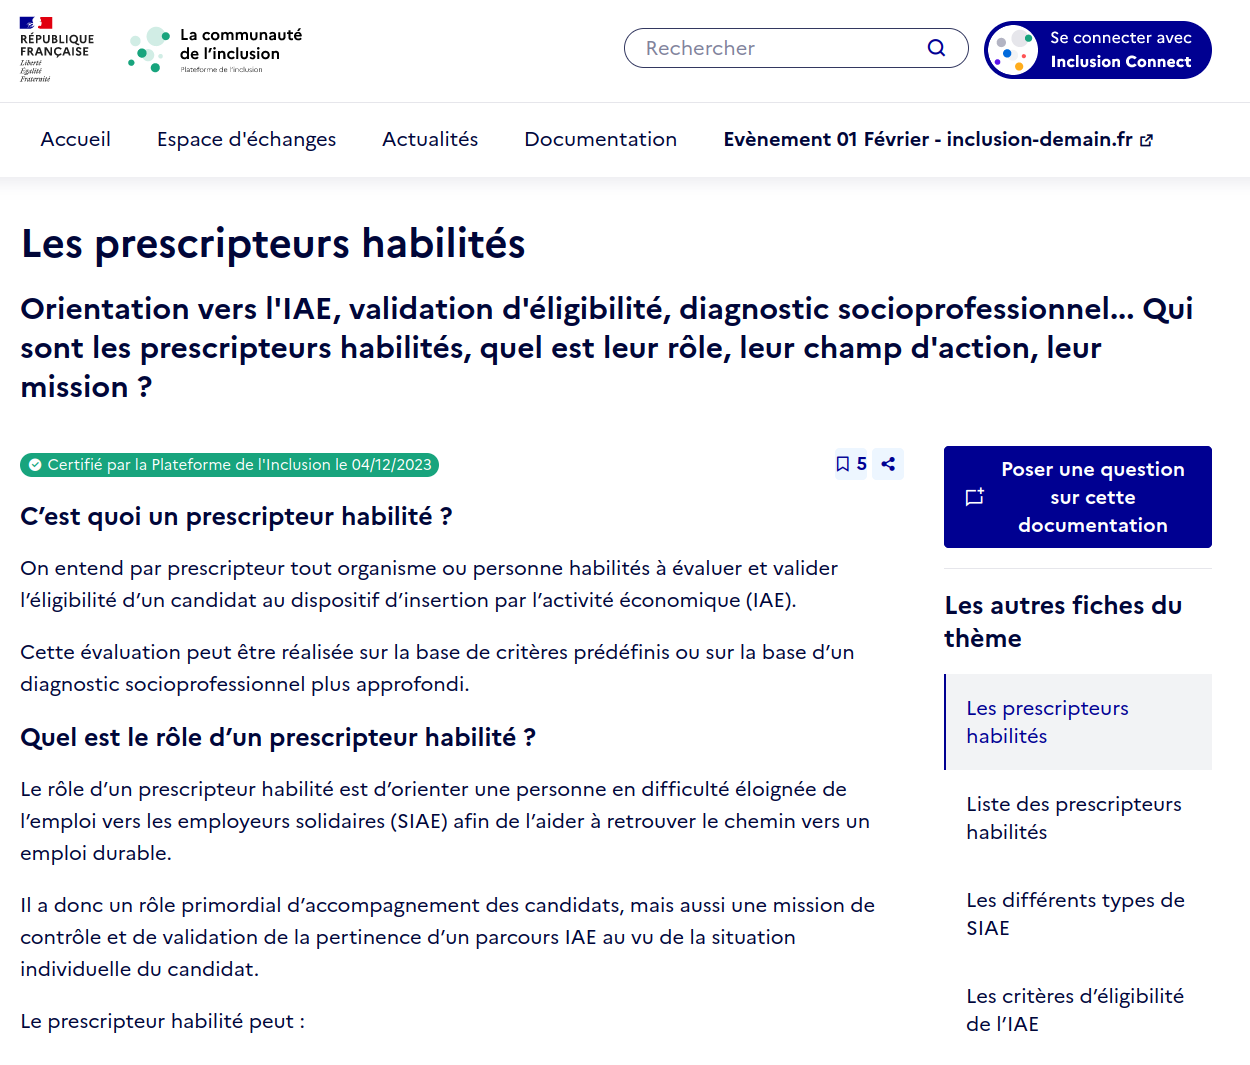
\includegraphics[width=\textwidth]{Images/communaute-documentation-fiche.png}
\end{frame}

\begin{frame}{L'espace d'échanges\hfill\href{https://github.com/ellmetha/django-machina/}{\textbf{[django-machina]}}}
    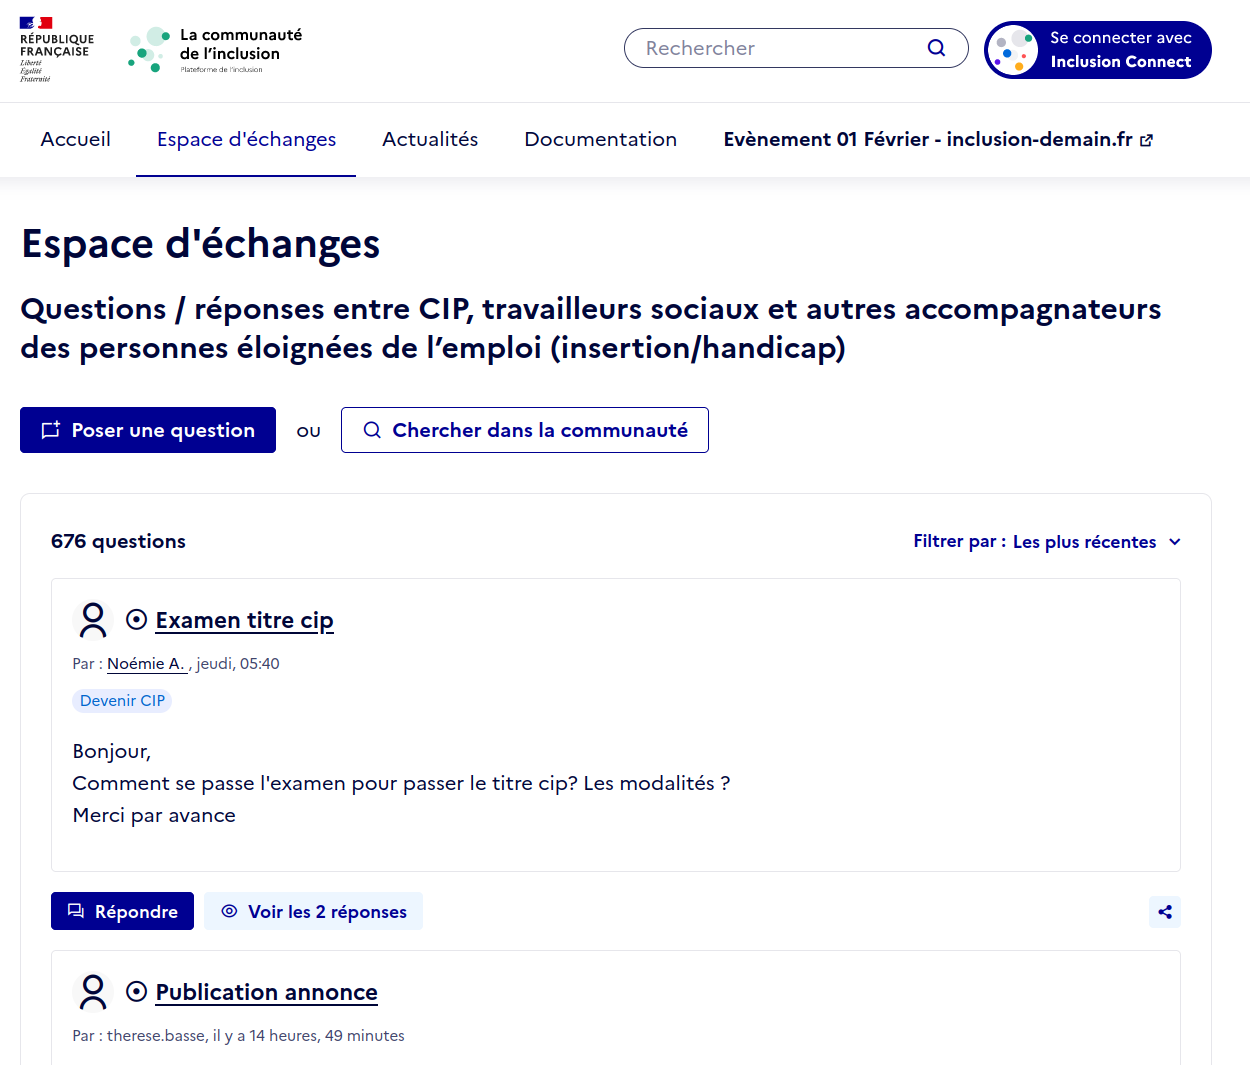
\includegraphics[width=\textwidth]{Images/communaute-espace-echanges.png}
\end{frame}

\begin{frame}{\texttt{Topic} et ses \texttt{Post}s\hfill\href{https://github.com/ellmetha/django-machina/}{\textbf{[django-machina]}}}
    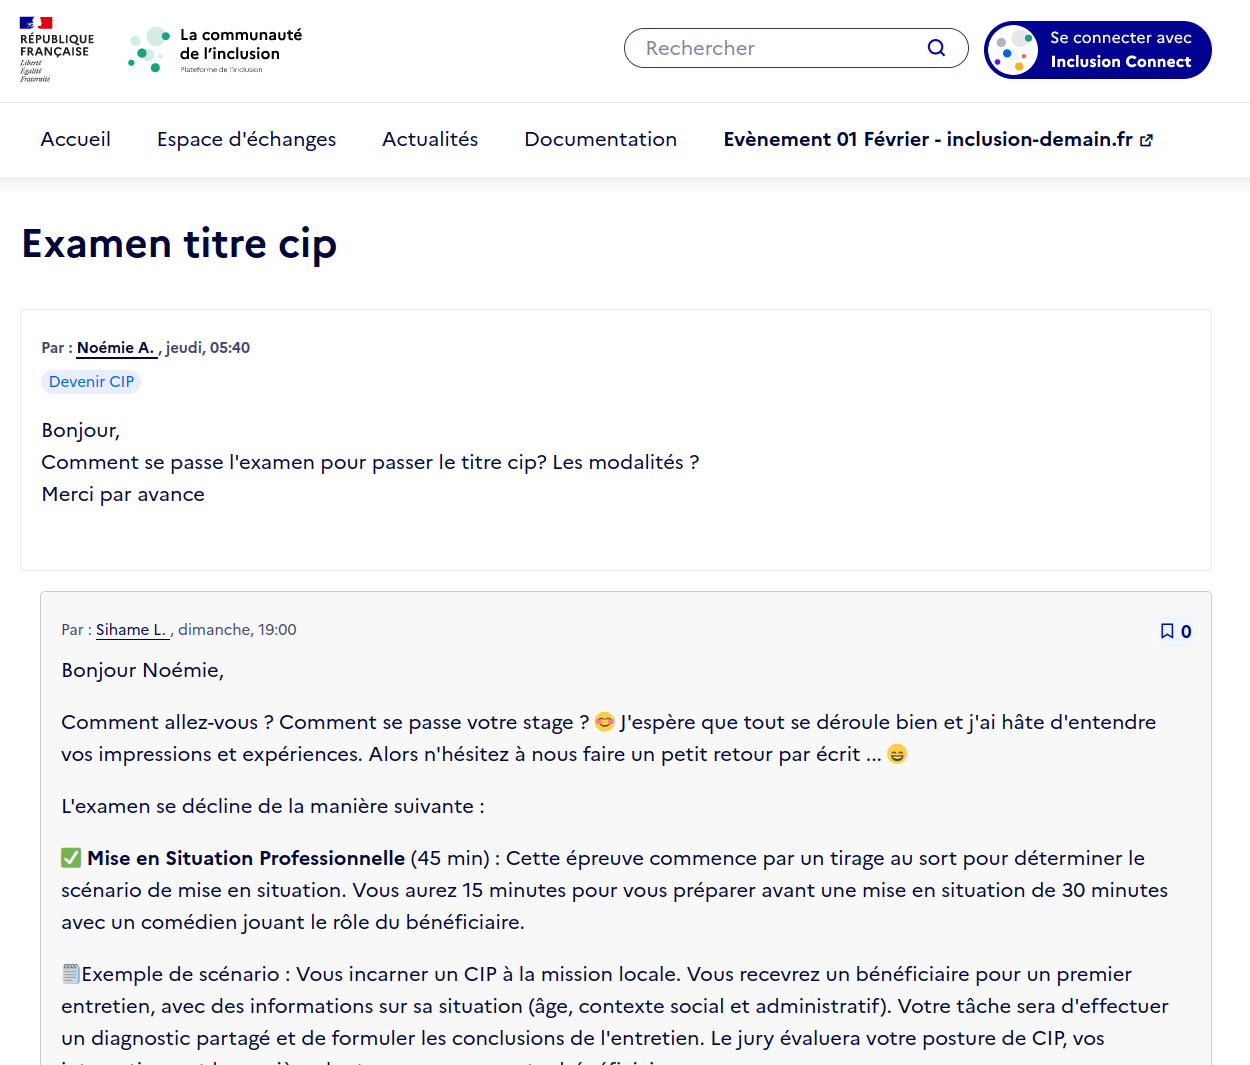
\includegraphics[width=\textwidth]{Images/communaute-topic.png}
\end{frame}

\begin{frame}{Le modèle de données à chercher}
    Construit avec \href{https://github.com/ellmetha/django-machina/}{\textbf{django-machina}} \emoji{folded-hands}
    \vspace{10pt}
    \\
    \pause
    Modèles de données principaux :
    \begin{itemize}
        \item \texttt{\textbf{Post}}: messages des utilisateurs
        \pause
        \item \texttt{\textbf{Topic}}: groupement de messages sur un sujet
        \pause
        \item \texttt{\textbf{Forum}}: ensemble de \texttt{\textbf{Topic}}
            \begin{itemize}
                \item les fiches thématiques sont des \texttt{\textbf{forum}}
                    avec une description écrite par l'équipe de la communauté
            \end{itemize}
    \end{itemize}
\end{frame}

\begin{frame}{La recherche en image}
    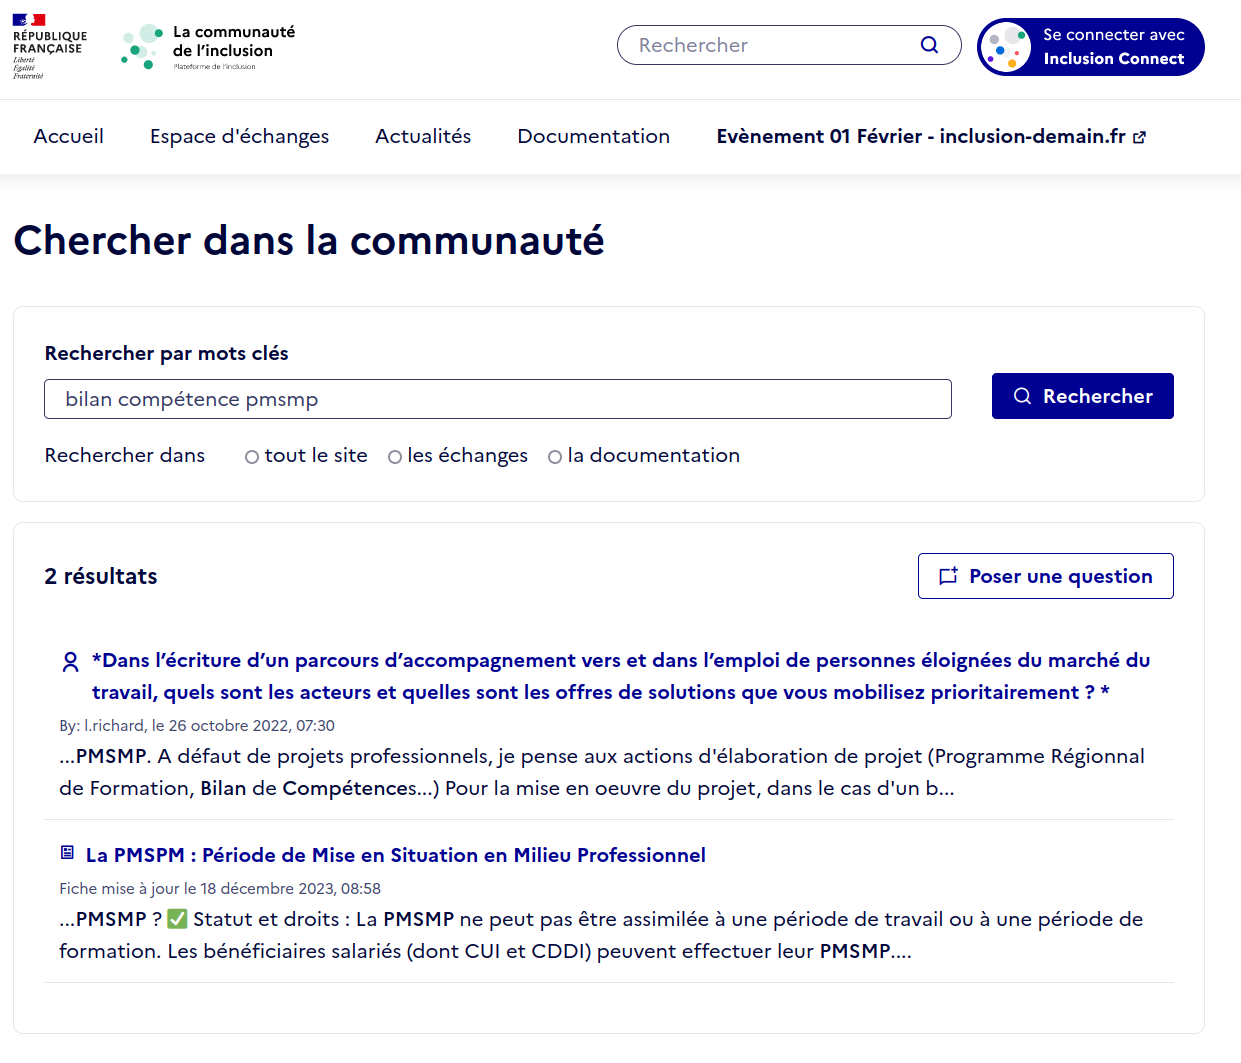
\includegraphics[width=\textwidth]{Images/communaute-search.png}
\end{frame}

%----------------------------------------------------------------------------------------
%	 SECTION 2
%----------------------------------------------------------------------------------------
\section{Whoosh et ses limites} % Section title slide, unnumbered

\begin{frame}{La recherche dans \href{https://github.com/ellmetha/django-machina/}{\textbf{[django-machina]}}}
    Basée sur \href{https://github.com/django-haystack/django-haystack}{\textbf{django-haystack}}:
    \vspace{15pt}
    \\
    \foreignquote{english}{Haystack provides modular search for Django. It
    features a unified, familiar API that allows you to plug in different
    search backends (such as Solr, Elasticsearch, Whoosh, Xapian, etc.) without
    having to modify your code.}
    \vspace{15pt}
    \\
    \href{https://github.com/mchaput/whoosh}{\textbf{Whoosh}}:
    \vspace{15pt}
    \\
    \foreignquote{english}{Whoosh is a fast, pure Python search engine library.
    The primary design impetus of Whoosh is that it is pure Python. }
\end{frame}

\begin{frame}{Whoosh: fonctionnement}
    \begin{itemize}
        \item Construction du fichier d'index sur le disque \hfill [15 secondes]

        \begin{itemize}
            \item Au déploiement
            \item Hebdomadaire
        \end{itemize}

        \item Mise à jour quotidienne \hfill [5 secondes]

    \end{itemize}
\end{frame}

\begin{frame}[fragile]
    \frametitle{Whoosh: intégration \hfill [\texttt{Post}]}

    \begin{minted}[bgcolor=LightGray,fontsize=\footnotesize]{python}
from haystack.indexes import Indexable, SearchIndex

class PostIndex(SearchIndex, Indexable):
    text = indexes.CharField(...)
    # Other fields to index.

    def get_model(self):
        return Post

    def index_queryset(self, using=None):
        return self.get_model().filter(...)

    # Boilerplate details.
    \end{minted}
\end{frame}

\begin{frame}[fragile]
    \frametitle{Whoosh: intégration \hfill [\texttt{Forum}]}

    \begin{minted}[bgcolor=LightGray,fontsize=\footnotesize]{python}
from haystack.indexes import Indexable, SearchIndex

class ForumIndex(SearchIndex, Indexable):
    text = indexes.CharField(...)
    # Other fields to index.

    def get_model(self):
        return Forum

    def index_queryset(self, using=None):
        return self.get_model().filter(...)

    # Boilerplate details.
    \end{minted}
\end{frame}

\begin{frame}{Whoosh: pourquoi changer ?}
    \begin{enumerate}
        \item Mise en avant des fiches thématiques (écrites par l'équipe) difficile
        \pause
        \item Whoosh sans activité depuis 2 ans, son futur est incertain
            \begin{itemize}
                \pause
                \item Utilisation de travis-ci
                \pause
                \item Plusieurs \textit{warnings} de dépreciation sur les
                    versions récentes de Python
                \pause
                \item
                    \href{https://github.com/Sygil-Dev/whoosh-reloaded}{\textit{Fork}
                    très récent de l'employeur}
                \pause
            \end{itemize}
        \item Les autres moteurs de recherche \texttt{Solr},
            \texttt{Xapian} et \texttt{ElasticSearch} nécessitent une
            infrastructure spécifique
        \pause
        \item Montée à l'échelle (partage de l'index entre différentes machines)
        \pause
        \item Problèmes gestion d'index dans les tests (isolation)
    \end{enumerate}
\end{frame}

%----------------------------------------------------------------------------------------
%	 SECTION 3
%----------------------------------------------------------------------------------------
\section{Introduction à la recherche texte plein avec PostgreSQL} % Section title slide, unnumbered

\begin{frame}{Recherche texte plein : vue d'ensemble}
    \begin{enumerate}
        \item Analyser les \textbf{documents} et en extraire les lexèmes\newline
            (contenus dans un \texttt{tsvector})
        \item \textbf{Pondérer} les sources
        \item Analyser la \textbf{requête} et en extraire les lexèmes\newline
            (interprétation de la syntaxe de recherche)
        \item \textbf{Classer} les résultats (\textit{cover density ranking})
        \item Extraire les \textbf{parties du document} correspondant à la recherche
    \end{enumerate}
\end{frame}

\begin{frame}[fragile]{Analyser les documents}
    Extraire et repérer les lexèmes du document
    \begin{minted}[bgcolor=LightGray,fontsize=\footnotesize]{sql}
SELECT to_tsvector(
    'french', -- config
    'Portez ce vieux whisky au juge blond qui fume.'
);
 to_tsvector
---------------------------------------------------------
 'blond':7 'fum':9 'jug':6 'port':1 'vieux':3 'whisky':4
(1 row)
    \end{minted}
\end{frame}

\begin{frame}[fragile]{Pondérer les sources}
    Aggréger les \texttt{Topic}s et les \texttt{Post}s, en attribuant plus de poids au titre
    \begin{minted}[bgcolor=LightGray,fontsize=\footnotesize]{sql}
SELECT (
    setweight(
        to_tsvector('french', topic.subject),
        'A'
    ) || setweight(
        to_tsvector('french', string_agg(post.content, ' ')),
        'C'
    )
) AS content_ts
FROM forum_conversation_topic topic
LEFT JOIN forum_conversation_post post
    ON topic_id = forum_conversation_topic.id
GROUP BY forum_conversation_topic.id;
    \end{minted}
\end{frame}

\begin{frame}[fragile]{Analyser la requête}
    Interpréter les termes de recherche, notamment les combinaisons (\texttt{ou}, \texttt{et}, \texttt{suivi de}, etc.)
    \begin{minted}[bgcolor=LightGray,fontsize=\footnotesize]{sql}
SELECT websearch_to_tsquery(
    'french', -- config
    'portez au juge'
);

 websearch_to_tsquery
------------------
 'port' & 'jug'
(1 row)
    \end{minted}
\end{frame}

\begin{frame}[fragile]{Analyser la requête}
    Exemple : \textbf{juge} \texttt{suivi de} \textbf{blond}
    \begin{minted}[bgcolor=LightGray,fontsize=\footnotesize]{sql}
SELECT websearch_to_tsquery(
    'french', -- config
    '"juge blond"'
);

 websearch_to_tsquery
------------------
 'jug' <-> 'blond'
(1 row)
    \end{minted}

    \texttt{<->} : \textit{Constructs a phrase query, which matches if the two input queries match at successive lexemes}
\end{frame}

\begin{frame}[fragile]{Classer les résultats}
    Mesurer la pertinence du contenu par rapport à la recherche
    \begin{minted}[bgcolor=LightGray,fontsize=\footnotesize]{sql}
SELECT ts_rank_cd(
    content_ts,
    websearch_to_tsquery('french', 'portez au juge')
) AS rank
FROM search_commonindex
ORDER BY 1 DESC
LIMIT 1;

   rank
-----------
 1.1416667
(1 row)
    \end{minted}
\end{frame}

\begin{frame}[fragile]{Parties du document pertinentes}
Mettre en avant comment la requête correspond au document
    \begin{minted}[bgcolor=LightGray,fontsize=\footnotesize]{sql}
SELECT ts_headline(
    'french', -- config
    'Voici une démonstration sur un texte plus long. '
    'L''idée est de mettre en avant les passages correspondant à '
    'la recherche. Par exemple : Portez donc ce vieux whisky au '
    'jeune juge blond qui fume. Notons que PostgreSQL ne donne '
    'qu''une partie intéressante du document.',
    websearch_to_tsquery('french', 'portez au juge')
);

                             ts_headline
------------------------------------------------------------------
<b>Portez</b> donc ce vieux whisky au jeune <b>juge</b> blond qui [...]
(1 row)
    \end{minted}
\end{frame}

\begin{frame}{Recherche texte plein : vue d'ensemble}
    \begin{enumerate}
        \item Analyser les \textbf{documents} et en extraire les lexèmes\newline
            (contenus dans un \texttt{tsvector})
        \item Analyser la \textbf{requête} et en extraire les lexèmes\newline
            (interprétation de la syntaxe de recherche)
        \item \textbf{Pondérer} les sources
        \item \textbf{Classer} les résultats (\textit{cover density ranking})
        \item Extraire les \textbf{parties du document} correspondant à la recherche
    \end{enumerate}
\end{frame}

%----------------------------------------------------------------------------------------
%	 SECTION 4
%----------------------------------------------------------------------------------------

\section{Intégration de la recherche PostgreSQL avec Django}

\begin{frame}{Avertissement}
    \begin{alertblock}{Modèles et tables simplifiées} Les modèles, tables et
        données des exemples à venir sont simplifiés pour faciliter la
        présentation.\par
        En cas de doute, il convient de suivre les liens vers le
        code en source libre présents dans chaque diapositive.
	\end{alertblock}
\end{frame}

\begin{frame}[fragile]{Index de recherche}
    Construction de l'index de recherche \hfill [150 ms] \href{https://github.com/gip-inclusion/itou-communaute-django/blob/b19e70216affb2e27d38f946ce9a9500ffa7be35/lacommunaute/search/migrations/0001_initial.py}{[code]}
    \begin{minted}[bgcolor=LightGray,fontsize=\footnotesize]{sql}
CREATE MATERIALIZED VIEW search_commonindex AS (
    SELECT
        topic.subject, string_agg(post.content, ' ') AS content,
        (setweight(to_tsvector('french', topic.subject), 'A')
            || setweight(
                to_tsvector('french',
                    string_agg(post.content, ' ')), 'C')
        ) AS content_ts,
    FROM forum_conversation_topic topic -- ...
    UNION ALL
    SELECT
        name, description,
        (setweight(to_tsvector('french', name), 'A')
            || setweight(to_tsvector('french', description)), 'B')
    FROM forum_forum -- ...
);
    \end{minted}
\end{frame}

\begin{frame}[fragile]{Mise à jour de l'index de recherche}
    Toutes les 10 minutes \hfill [10 ms] \href{https://github.com/gip-inclusion/itou-communaute-django/blob/b19e70216affb2e27d38f946ce9a9500ffa7be35/clevercloud/rebuild_index.sh}{[code]}
    \begin{minted}[bgcolor=LightGray,fontsize=\footnotesize]{sql}
REFRESH MATERIALIZED VIEW search_commonindex;
    \end{minted}
\end{frame}

\begin{frame}[fragile]{Intégration avec Django}
    Le modèle Django \hfill  \href{https://github.com/gip-inclusion/itou-communaute-django/blob/b19e70216affb2e27d38f946ce9a9500ffa7be35/lacommunaute/search/models.py}{[code]}
    \begin{minted}[bgcolor=LightGray,fontsize=\footnotesize]{python}
from django.contrib.postgres.search import SearchVectorField
from django.db import models

class CommonIndex(models.Model):
    subject = models.CharField(...)
    content = models.TextField(...)
    content_ts = SearchVectorField(...)

    class Meta:
        managed = False
    \end{minted}
\end{frame}

\begin{frame}[fragile]{Intégration avec Django}
    La vue Django \hfill \href{https://github.com/gip-inclusion/itou-communaute-django/blob/b19e70216affb2e27d38f946ce9a9500ffa7be35/lacommunaute/search/views.py}{[code]}
    \begin{minted}[bgcolor=LightGray,fontsize=\footnotesize]{python}
class SearchView(FormMixin, ListView):
    def get_queryset(self):
        queryset = super().get_queryset()
        q = self.get_form().cleaned_data["q"]
        search_query = SearchQuery(
            q, config="french", search_type="websearch"
        )
        return ( # Pardon the indentation, must fit on a slide ;)
    queryset
    .annotate(rank=SearchRank(F("content_ts"), search_query))
    .filter(rank__gte=0.01)
    .order_by("-rank")
    .annotate(headline=SearchHeadline(
        "content", search_query, config="french")
    ))
    \end{minted}
\end{frame}

%----------------------------------------------------------------------------------------
%	 SECTION 4
%----------------------------------------------------------------------------------------

\section{Conclusion}

\begin{frame}{Comment aller plus loin?}
    \begin{itemize}
        \item Mise à jour partielle de l'index de recherche avec des
            \texttt{TRIGGER}s lors de la modification des \texttt{Forum}s SQL,
            des \texttt{Topic}s et des \texttt{Post}s.
            \begin{itemize}
                \item [+] Rapidité d'indexation
                \item [+] Fraîcheur du contenu de la recherche
                \item [-] Performance du site
                \item [-] Complexité
            \end{itemize}
        \pause
        \item Suivi des recherches avec Matomo pour évaluer la pertinence des résultats
    \end{itemize}
\end{frame}

\begin{frame}[focus]
    Merci de votre attention
    \\
    \vspace{20pt}
    \rule{\textwidth}{1pt}
    \\
    \vspace{30pt}
    Avez-vous des questions ?
\end{frame}

%------------------------------------------------

% \begin{frame}[plain]{Plain Slide}
% 	This is a slide with the plain style and it is numbered.
% \end{frame}

%------------------------------------------------

% \begin{frame}[t]
% 	This slide has an empty title and is aligned to top.
% \end{frame}

%------------------------------------------------

% \begin{frame}[noframenumbering]{No Slide Numbering}
% 	This slide is not numbered and is citing reference \cite{knuth74}.
% \end{frame}

%------------------------------------------------

% \begin{frame}{Typesetting and Math}
% 	The packages \texttt{inputenc} and \texttt{FiraSans}\footnote{\url{https://fonts.google.com/specimen/Fira+Sans}}\textsuperscript{,}\footnote{\url{http://mozilla.github.io/Fira/}} are used to properly set the main fonts.
% 	\vfill
% 	This theme provides styling commands to typeset \emph{emphasized}, \alert{alerted}, \textbf{bold}, \textcolor{example}{example text}, \dots
% 	\vfill
% 	\texttt{FiraSans} also provides support for mathematical symbols:
% 	\begin{equation*}
% 		e^{i\pi} + 1 = 0.
% 	\end{equation*}
% \end{frame}


%------------------------------------------------

% \begin{frame}{Blocks}
% 	These blocks are part of 1 slide, to be displayed consecutively.
% 	\begin{block}{Block}
% 		Text.
% 	\end{block}
% 	\pause % Automatically creates a new "page" split between the above and above + below
% 	\begin{alertblock}{Alert block}
% 		Alert \alert{text}.
% 	\end{alertblock}
% 	\pause % Automatically creates a new "page" split between the above and above + below
% 	\begin{exampleblock}{Example block}
% 		Example \textcolor{example}{text}.
% 	\end{exampleblock}
% \end{frame}

%------------------------------------------------

% \begin{frame}{Columns}
% 	\begin{columns}
% 		\column{0.5\textwidth}
% 			This text appears in the left column and wraps neatly with a margin between columns.

% 		\column{0.5\textwidth}
% 			\includegraphics[width=\linewidth]{Images/placeholder.jpg}
% 	\end{columns}
% \end{frame}

%------------------------------------------------

% \begin{frame}{Lists}
% 	\begin{columns}[T, onlytextwidth] % T for top align, onlytextwidth to suppress the margin between columns
% 		\column{0.33\textwidth}
% 			Items:
% 			\begin{itemize}
% 				\item Item 1
% 				\begin{itemize}
% 					\item Subitem 1.1
% 					\item Subitem 1.2
% 				\end{itemize}
% 				\item Item 2
% 				\item Item 3
% 			\end{itemize}

% 		\column{0.33\textwidth}
% 			Enumerations:
% 			\begin{enumerate}
% 				\item First
% 				\item Second
% 				\begin{enumerate}
% 					\item Sub-first
% 					\item Sub-second
% 				\end{enumerate}
% 				\item Third
% 			\end{enumerate}

% 		\column{0.33\textwidth}
% 			Descriptions:
% 			\begin{description}
% 				\item[First] Yes.
% 				\item[Second] No.
% 			\end{description}
% 	\end{columns}
% \end{frame}

%------------------------------------------------

% \begin{frame}{Table}
% 	\begin{table}
% 		\centering % Centre the table on the slide
% 		\begin{tabular}{l c}
% 			\toprule
% 			Discipline & Avg. Salary \\
% 			\toprule
% 			\textbf{Engineering} & \textbf{\$66,521} \\
% 			Computer Sciences & \$60,005\\
% 			Mathematics and Sciences & \$61,867\\
% 			Business & \$56,720\\
% 			Humanities \& Social Sciences & \$56,669\\
% 			Agriculture and Natural Resources & \$53,565\\
% 			Communications & \$51,448\\
% 			\midrule
% 			\textbf{Average for All Disciplines} & \textbf{\$58,114}\\
% 			\bottomrule
% 		\end{tabular}
% 	\caption{Table caption}
% 	\end{table}
% \end{frame}

%------------------------------------------------

% \begin{frame}[focus]
% 	Thanks for using \textbf{Focus}!
% \end{frame}

%----------------------------------------------------------------------------------------
%	 CLOSING/SUPPLEMENTARY SLIDES
%----------------------------------------------------------------------------------------

% \appendix

%\begin{frame}{References}
%	\nocite{*} % Display all references regardless of if they were cited
%	\bibliography{example.bib}
%	\bibliographystyle{plain}
%\end{frame}

%------------------------------------------------

% \begin{frame}{Backup Slide}
% 	This is a backup slide, useful to include additional materials to answer questions from the audience.
% 	\vfill
% 	The package \texttt{appendixnumberbeamer} is used to refrain from numbering appendix slides.
% \end{frame}

%----------------------------------------------------------------------------------------

\end{document}
